\chapter{Zagotavljanje varnosti v sodelovalni aplikaciji z robotom Motoman HC10DT}%

\begin{mdframed}[backgroundcolor=green!20, shadow=true,roundcorner=8pt]
	\vspace{-0.35cm}
	
	\section{Cilj vaje}
	
	Pri tej vaji boste spoznali različne varnostne funkcije, ki se jih lahko implementira v konceptu sodelovalne aplikacije. Varnostne elemente boste uporabili v povezavi s sodelujočim robotom Motoman HC10DT proizvajalca Yaskawa. V prvem delu vaje boste definirali varnostno ovojnico prijemala in varnostno območje objekta, ki se nahaja v delovnem prostoru robota, nato pa testirali delovanje preprečevanja trka med robotom in objektom. V drugem delu vaje boste implementirali aplikacijo pobiranja palete laboratorijskih epruvet in preizkusili varnostna mehanizma varnega odmika in nadzorovanja sile. Tretji del zajema uporabo laserskega skenerja proizvajalca SICK za definiranje dveh varnostnih območij. Na podlagi informacije o lokaciji uporabnika boste ustrezno prilagodili hitrost gibanja robota.
	
\end{mdframed}

\section{Sodelovanje človek--robot}

Sodelovanje med človekom in robotom združuje lastnosti obeh akterjev: človeško inteligenco, prilagodljivost in sposobnost rokovanja z nedeterminiranimi materiali ter robotsko vzdržljivost, natančnost in moč. Pri tem je neizogibno, da človek in robot opravljata nalogo v neposredni bližini. Tehnično priporočilo standardu ISO/TS 15066:2016 predpisuje zahteve za različne načine sodelovanja. Pomembna je tudi ocena tveganja celotnega sistema (ta vključuje robota, prijemalo, obdelovanec, periferijo, človeka), s katero identificiramo potencialno nevarne situacije ter rešitve, kako se jim izogniti.

Skupno delovanje človeka in robota lahko razdelimo na tri dele:
\begin{itemize}
	\item \textbf{soobstoj} -- robot in delavec sta prisotna v skupnem prostoru, robot je ločen od delavca, ne more priti do kontakta med robotom in delavcem,
	\item \textbf{kooperacija} -- robot in delavec si delita delovni prostor, naloge izvajata simultano na ločenih objektih, interakcija z robotom prek skupnega delovnega prostora, kjer si izmenjujeta delovne objekte,
	\item  \textbf{sodelovanje} -- robot in delavec si delita delovni prostor, nalogo izvajata na simultano na skupnem objektu.
\end{itemize}


\begin{figure}[!hbt]
	\centering
	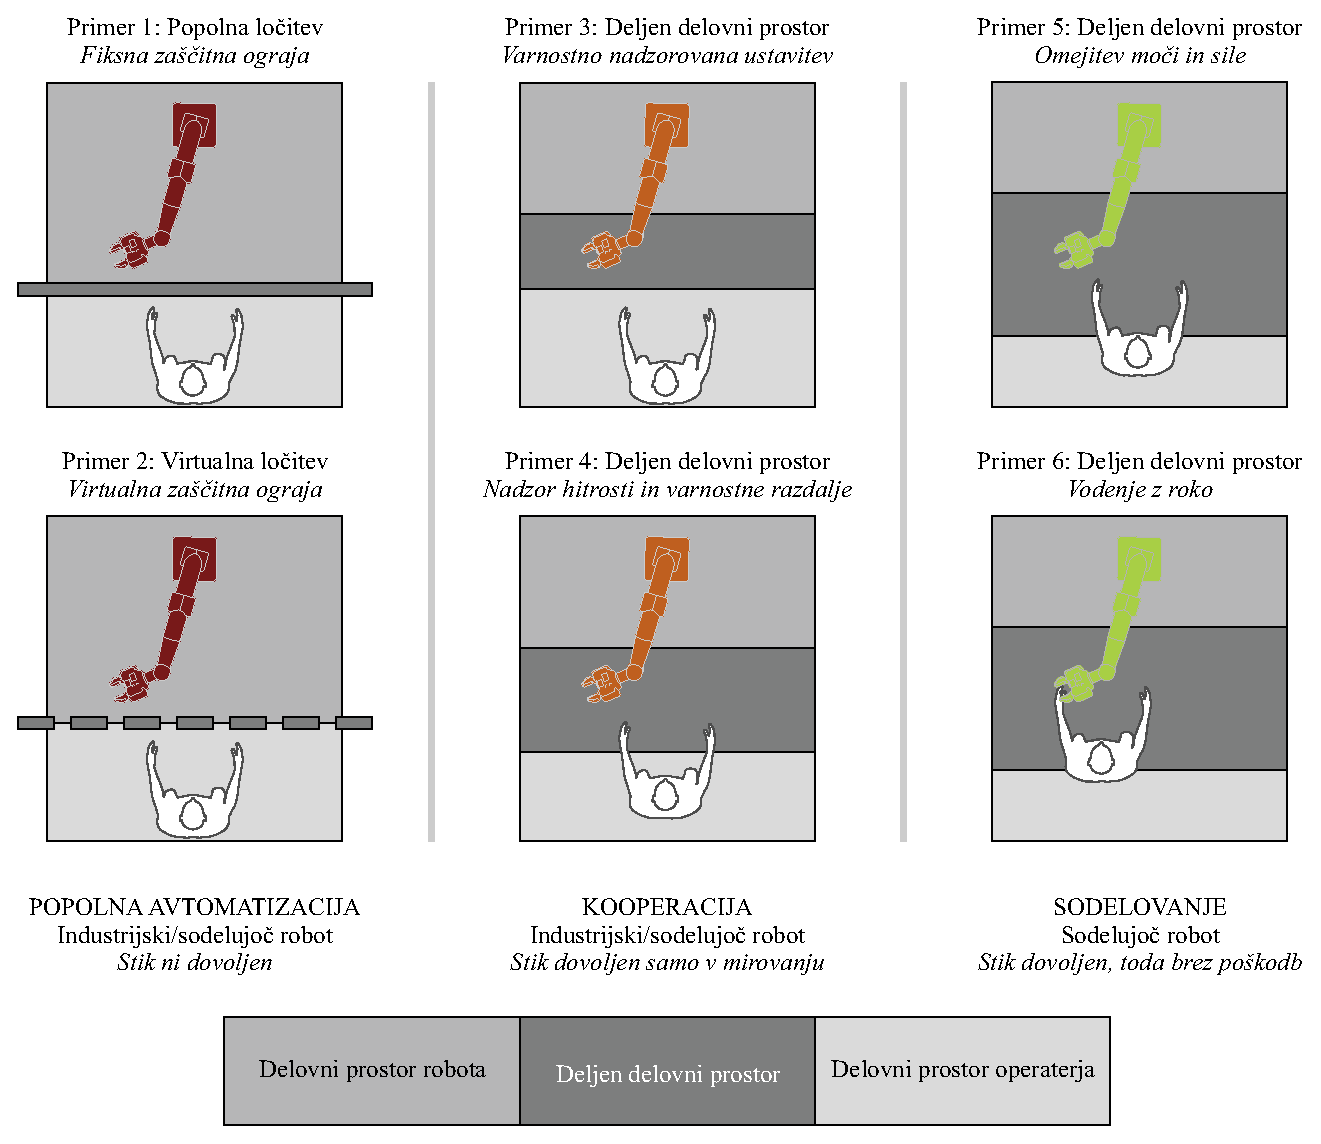
\includegraphics[width=\textwidth]{hc10_sodelovanje.eps}
	\caption{Primeri različnih načinov sodelovanja človeka in robota}
	\label{fig:hc10_sodel}
\end{figure}


Za zagotavljanje varnosti operaterja mora imeti robot implementirano vsaj eno izmed štirih kategorij varnosti:
\begin{itemize}
	\item \textbf{varnostno nadzorovana ustavitev} -- v primeru nevarne situacije se robot ustavi (motorji so prižgani),
	\item \textbf{vodenje z roko}  -- operater lahko ročno vodi robota, enostavnejše programiranje in izvajanje aplikacij,
	\item \textbf{nadzor hitrosti in varnostne razdalje} -- hitrost robota se prilagaja glede na oddaljenost človeka od robota (različne cone hitrosti, bližje kot je operater robotu, manjša je hitrost), potrebni dodatni senzorji (laserski skenerji, svetlobne zavese, ...)
	\item \textbf{omejitev moči in sile} -- robot deluje z ustrezno močjo, da v primeru nehotenega trka z operaterjem ne pride do poškodbe, ISO/TS 15066:2016 podaja ustrezne sile/pritiske za posamezna področja človeškega telesa, kompromis med hitrostjo in nosilnostjo robota.
\end{itemize}


\section{Struktura sistema}
Robotski sistem sestavlja sodelujoči robot Yaskawa Motoman HC10DT s krmilnikom YRC1000, pneumatsko robotsko prijemalo Zimmer MGP812N ter laserski skener SICK TIM310-1130000. Celotna konfiguracija je predstavljena na sliki \ref{fig:hc10_sistem}.

\begin{figure}[!hbt]
	\centering
	\includegraphics[width=0.9\textwidth]{hc10_sistem.eps}
	\caption{Robotski sistem}
	\label{fig:hc10_sistem}
\end{figure}

\subsection{Motoman HC10DT}

Robot je predstavnik sodelujočih robotov, ki so narejeni za varno delo skupaj s človekom brez dodatnih varnostnih elementov (varnostnih ograj, svetlobnih zaves ...), seveda v skladu z analizo tveganja. Robotska roka je antropomorfne oblike s 6 prostostnimi stopnjami. Posamezni sklep robota je opremljen s senzorjem navora, ki na nivoju sklepa meri interakcijo robota z okolico. Robota se lahko premika z roko, za shranjevanje ukazov pa se lahko uporablja vmesnik na vrhu robota, kar omogoča prihranek časa pri programiranju robota.

Osnovni podatki robotske roke so podani v tabeli \ref{tab:hc10}.

\begin{table}
	\centering
	\caption{Specifikacije robota Yaskawa Motoman HC10DT} \label{tab:hc10}
	\begin{tabular}{|lr|c|}
		\hline   Tip &  & HC10DT \\
		\hline Doseg & & $1,2$ m \\
		\hline Nosilnost  & & $9$ kg \\
		\hline Hitrost vrha& & $1$ m/s \\
		\hline Hitrost vrha (varen način)& & $0,25$ m/s \\
		\hline Ponovljivost pozicioniranja& & $\pm 0.1$ mm \\
		\hline Maksimalna hitrost
		& Os 1 & $130$ $^\circ/s$ \\
		& Os 2 & $130$ $^\circ/s$ \\
		& Os 3 & $180$ $^\circ/s$ \\
		& Os 4 & $180$ $^\circ/s$ \\
		& Os 5 & $250$ $^\circ/s$ \\
		& Os 6 & $250$ $^\circ/s$ \\
		\hline Delovni prostor
		& Os 1 & $\pm180^\circ$\\
		& Os 2 & $\pm180^\circ$\\
		& Os 3 & $-5^\circ/+355^\circ$\\
		& Os 4 & $\pm180^\circ$\\
		& Os 5 & $\pm180^\circ$\\
		& Os 6 & $\pm180^\circ$\\
		\hline   Teža &  & $48$ kg \\
		\hline
	\end{tabular}
\end{table}

Robot lahko deluje v dveh načinih. Prvi je kot klasični industrijski manipulator, kjer je maksimalna hitrost vrha deklarirana na 1000~mm/s. V tem načinu je potrebno robota ločiti od delavcev z varnostnimi elementi (ograje, svetlovne zavese). Drugi način pa je kot sodelujoči robot. V tem načinu je hitrost vrha omejena na 250~mm/s. Pri tej hitrosti in deklarirani nosilnosti robot v primeru trka s človekom ne povzroči poškodbe (glede na specifikacije ISO/TS 15066:2016).

Robota se programira z uporabo ročne učne enote (slika \ref{fig:hc10_pendant}). Ta omogoča premikanje robota, upravljanje s prijemali, pisanje, popravljanje in poganjanje programov ter podobno.

\begin{figure}[!hbt]
	\centering
	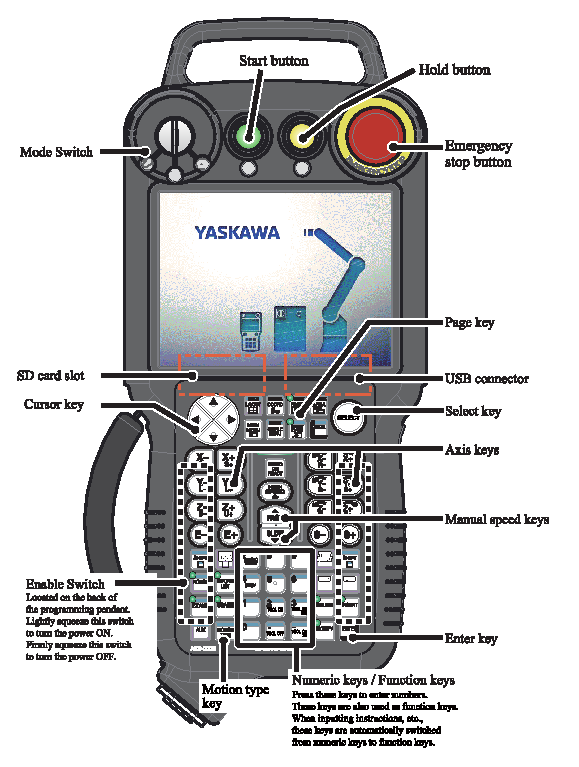
\includegraphics[width=0.9\textwidth]{hc10_pendant.eps}
	\caption{Ročna učna enota}
	\label{fig:hc10_pendant}
\end{figure}

Robot HC10DT je opremljen z integriranim varnostnim krmilnikom FSU (Functional Safety Unit), ki omogoča različne varnostne funkcije. S FSU se lahko nastavi dovoljena območja gibanja posameznega sklepa, maksimalne dovoljene hitrosti za posamezni sklep ter za vrh robota, ter se definira različna območja delovanja (območje, ki ga robot ne sme zapustiti, območje, v katerega robot ne sme vstopiti, ravnine, ki omejujejo gibanje robota).

\subsection{Laserski skener SICK TIM310}

Laserski skener SICK TIM310 detektira objekte v različnih področjih glede na odboj laserskega žarka. Doseg skeniranje je do 4~m. Senzor podpira nastavitev treh delno prekrivajočih področij enake oblike vendar različnih velikosti (glej sliko \ref{fig:hc10_sick}). Oblike področij so  v naprej definirane ali pa jih uporabnik nastavi sam. Senzor sporoča v katerem polju se nahaja objekt preko digitalnih linij (vsako področje ima ločeno linijo), zato je z robotskim krmilnikom (FSU) povezan preko digitalnih vhodov.

\begin{figure}[!hbt]
	\centering
	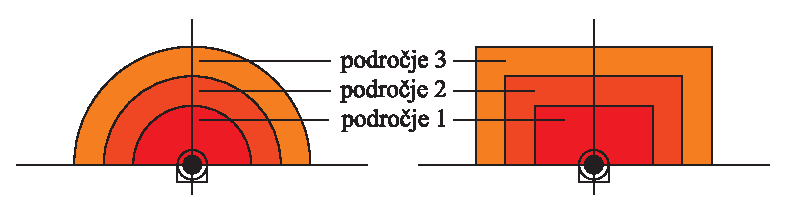
\includegraphics[width=0.9\textwidth]{hc10_podrocja.eps}
	\caption{Primera polkrožnega in pravokotnega področja zaznavanja senzorja}
	\label{fig:hc10_sick}
\end{figure}

Za nastavljanje področij in parametrov senzorja se uporablja program SOPAS. Ta omogoča nastavljanje oblike in velikosti področij, odzivni čas zaznave posameznega področja, velikost objektov, ki jih zanemari, in čas signaliziranja o detektiranem objektu.

\section{I. del: Definiranje varnostnega območja in ovojnice prijemala}

Na prirobnico robota je z adapterjem nameščeno pneumatsko prijemalo Zimmer MGP812N. S pravilno definicijo orodja robotski krmilnik upošteva dimenzije in parametre orodja za ustrezno izvajanje programa in nalog. Za namen laboratorijske vaje sta nastavljena dva vrha (kalibracijska špica in prsti za pobiranje palete), med katerima lahko izbiramo s kombinacijo tipk \textbf{SHIFT} + \textbf{COORD} (TOOL SEL). Nastavljeni orodji se nahajata pod številkama \textbf{15} - kalibracijska špica in \textbf{16} - prsti za pobiranje palete. Prste za pobiranje palete lahko upravljate v meniju \textbf{IN/OUT > General purpose output > \textit{Označite piko ob izhodu št. 1} > INTERLOCK + Select}.

\subsection*{Varnostna ovojnica prijemala}

Poleg vrha prijemala je potrebno nastaviti tudi varnostno ovojnico, ki robotskem krmilniku poda informacijo o velikosti in obliki celotnega orodja. Vsako orodje ima lahko pet prekrivajočih se ovojnic v obliki kapsule. Definiramo jih z dvema točkama in radijem. Točke so definirane v koordinatnem sistemu vrha robota, ki je prikazan na sliki \ref{fig:hc10_prirobnica}.

\begin{figure}[htbp]
	\centering
	\includegraphics[width=0.4\textwidth]{hc10_prirobnica.eps}
	\caption{Koordinatni sistem vrha robota Yaskawa Motoman HC10dt.}
	\label{fig:hc10_prirobnica}
\end{figure}

Orodju številka \textbf{16} določite parametre ovojnic z menijem \textbf{ROBOT > TOOL INTERFERE}, prijemalo pa izberite s tipko \textbf{Page}. Pri tem si pomagajte s sliko \ref{fig:hc10_ovoj1}. Skrajne lege ovojnic morate definirati glede na koordinatni sistem vrha robota. Ko vpišete parametre, ne pozabite parametrov shraniti z \textbf{READBACK > WRITE > YES}. V meniju \textbf{SAFETY FUNC. > OPERATION AREA MONITOR} si lahko ogledate grafični prikaz ovojnic, ki ste jih vpisali. Če katerakoli kapsula, ki ste jo določili, vstopi v varnostno področje, FSU sistem javi, da je prišlo do dotika z varnostnim področjem.

\begin{figure}[!hbt]
	\centering
	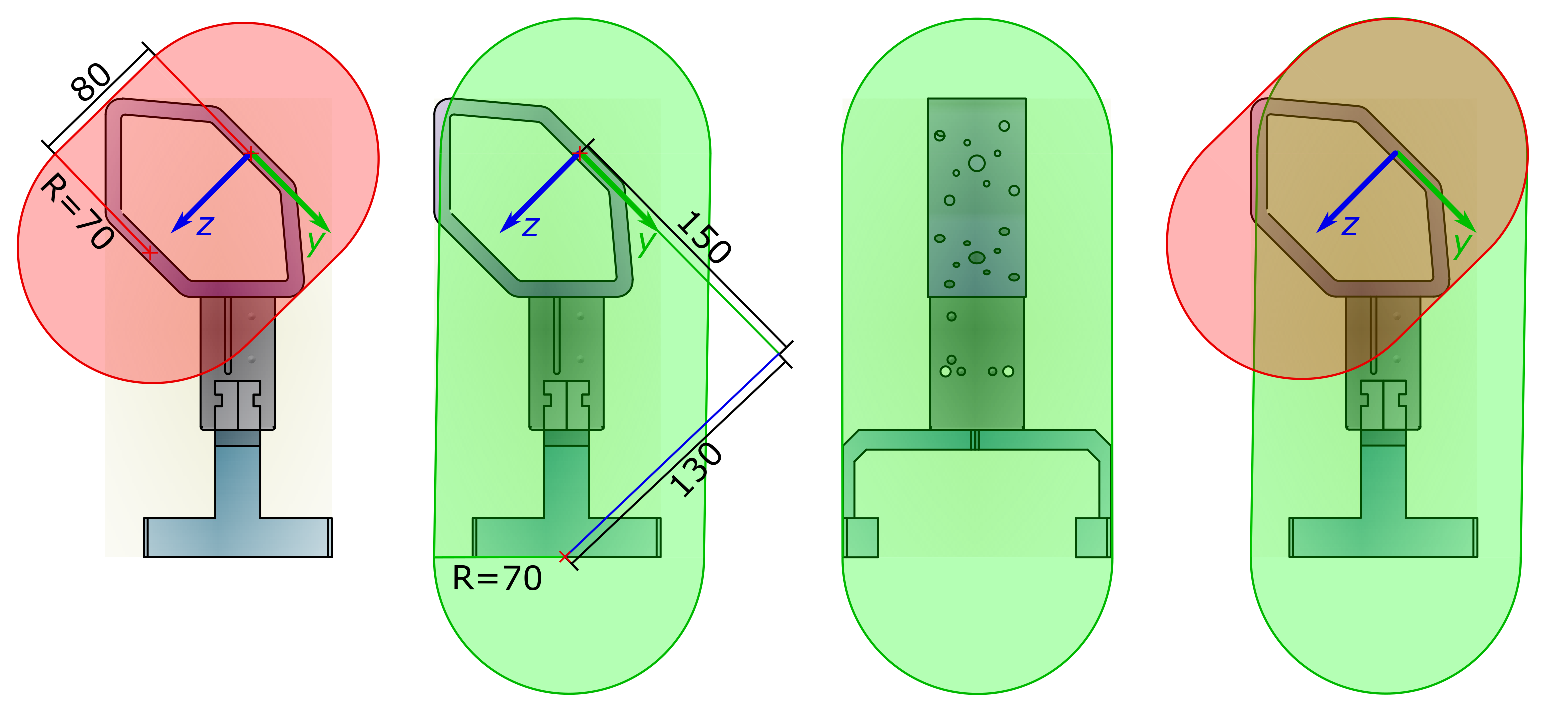
\includegraphics[width=\textwidth]{hc10_ovoj6.eps}
	\caption{Prikaz ovojnic (kapsul) okoli orodja. Označen koordinatni sistem predstavlja koordinatni sistem vrha robota.}
	\label{fig:hc10_ovoj1}
\end{figure}

\subsection*{Definiranje varnostnega območja}

V nadaljevanju preizkusite varnostni mehanizem uporabe navideznih varnostnih območij. Na mizo postavite kocko (pravokotno na koordinatni sistem baze), ki vam bo služila kot fizični model varnostnega območja. V meniju \textbf{SAFETY FUNC. > ROBOT RANGE LIMIT} boste vpisali podatke za varnostno območje v obliki kvadra. Primer parametrov je podan na sliki \ref{fig:hc10_ovoj3}. 

Kocko boste definirali s pomočjo kalibracijske špice na vrhu robota. Za izbiro kalibracijske špice hkrati pritisnite tipki \textbf{SHIFT + COORD (TOOL SEL)} in se pomaknite na orodje številka \textbf{15}. Meni zaprite s ponovnim pritiskom \textbf{SHIFT + COORD (TOOL SEL)}. Robot se v trenutni konfiguraciji z orodjem \textbf{15} težko premika, zato ga premaknite v začetno lego. To lahko naredite v meniju \textbf{ROBOT -> SECOND HOME POS}, tako da držite tipko \textbf{FWD}.

S kalibracijsko konico se premaknite v nasprotni ogljišči kocke ter njune koordinate preberite v meniju \textbf{ROBOT > CURRENT POSITION}. Preverite, da so koordinate podane v baznem koordinatnem sistemu (\textbf{COORDINATE} na bazni koordinatni sistem \textbf{BASE} - tipka \textbf{SELECT}). Koordinate si zapišite ali slikajte, nato pa odprite meni za nastavitev varnostnih območij - \textbf{SAFETY FUNC. > ROBOT RANGE LIMIT}.

Najprej preverite, da so vsa varnostna polja izklopljena (\textbf{INVALID} v stolpcu \textbf{STATUS}). Če niso, jih izklopimo - \textbf{Select}, da odpremo parametre varnostnega območja, polje \textbf{FILE VALID COND}  spremenimo v \textbf{INVALID}, nato pa spremembo shranimo. V polje ena lahko nato vpišemo svoje varnostno polje:

\begin{itemize}
	\item V polju \textbf{FILE NO.} je vpisana zaporedna številka polja.
	\item V polje \textbf{COMMENT} vpišete ime območja.
	\item V polju \textbf{ALARM} izberete možnost \textbf{ON(MOVE STOP)}. S tem izberete možnost, da se robot ustavi, ko vstopi v varnostno območje.
	\item V polju \textbf{MONITOR TARGET} izberete možnost \textbf{OUTSIDE}.
	\item V polju \textbf{SHAPE TYPE} izberete možnost \textbf{CUBOID} (oblika varnostnega območja bo kvader). Mere kvadra bodo določene z dvema skrajnima, diagonalno nasprotnima,  ogliščema, ki jih vpišete v polji  \textbf{POINT1} in \textbf{POINT2}.
\end{itemize}

\begin{figure}[!hbt]
	\centering
	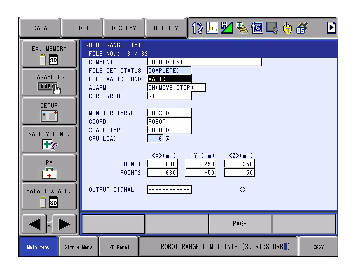
\includegraphics[width=0.7\textwidth]{hc10_ovoj3.eps}
	\caption{Parametri varnostnega področja}
	\label{fig:hc10_ovoj3}
\end{figure}

Na zadnje v polju \textbf{FILE VALID COND} izberete možnost \textbf{VALID}. S tem potrdite, da bo FSU enota preverjala trk med navideznim varnostnim področjem in ovojnicami robota z orodjem. Na seznamu varnostnih področij imate lahko namreč vpisanih več različnih področij, ki jih nato po potrebi vklapljate in izklapljate  v polju \textbf{FILE VALID COND}. Možnost \textbf{VALID} pomeni, da se bo trk preverjal, možnost \textbf{INVALID} pa pomeni, da FSU ne upošteva varnostnega področja pri analizi trka. Nastavitve potrdite z zaporedjem ukazov \textbf{Readback > Write > Yes > Confirm}.

\subsection*{Test preprečevanja trka med objekti}

Varnostne nastavitve preizkusite z orodjem št. 16. Orodje izberete tako, da pritisnete tipki \textbf{SHIFT} in \textbf{COORD} hkrati, nato pa se pomaknete na orodje št. 16. Nastavitev potrdite s ponovnim pritiskom tipk \textbf{SHIFT} in \textbf{COORD}. Z menijem \textbf{SAFETY FUNC. > OPERATION AREA MONITOR} izberete vizualni prikaz varnostnih področij in ovojnic robota. V oknu \textbf{Operation Area Monitor} najprej v polju \textbf{File No:} izberete številko vašega varnostnega področja. Z gumbi \textbf{Change Plane} izbirate pogled na robota in  varnostno območje. Premaknite robota tako, da ni v stiku z varnostnim območjem (recimo nad varnostno območje). Robota nato pomaknite navzdol, da bo prispel v stik z varnostnim področjem. Ko pride do trka, se v oknu \textbf{Operation Area Monitor} ovojnica, ki pride v stik z varnostnim področjem obarva z rdečo, kot je to prikazano na sliki \ref{fig:hc10_ovoj4}. Varnostna območja preizkusite z ročnim premikanjem robota.

\begin{figure}[!hbt]
	\centering
	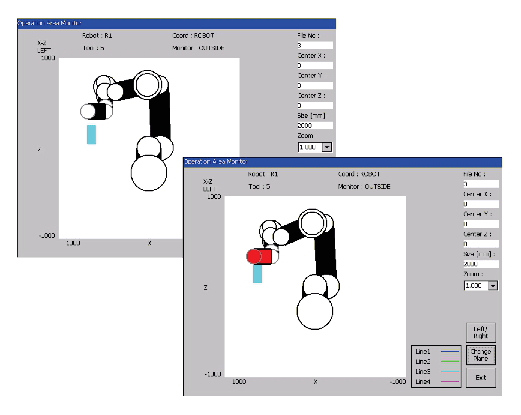
\includegraphics[width=0.9\textwidth]{hc10_ovoj4.eps}
	\caption{Prikaz trka med ovojnicami robota in orodja ter varnostnega področja (moder pravokotnik)}
	\label{fig:hc10_ovoj4}
\end{figure}

\section{II. del: Varnostni odmik robota} \label{poglavje2del_vaje}

FSU skrbi tudi za implementacijo varnostnega protokola omejtive moči in sile. V tem primeru je kontakt med robotom in uporabnikom dovoljen, saj robot v primeru detektiranja zunanje sile aktivira varnostno nadzorovano ustavitev. Ko uporabnik potrdi, da ni več neželjenega kontakta (restart gumb na petem segmentu), robot nadaljuje z opravljanjem naloge. Zunanja sila je ocenjena na podlagi primerjave izračunanih navorov v sklepih na podlagi trenutne lege robota (in znanih dinamičnih in kinematičnih parametrih robota) ter izmerjenimi navori s sklepnimi senzorji  navora. Razlike med navori se upoštevajo kot sklepni prispevki zunanjih sil, ki delujejo na robota (kontakt).

Robot ima implementiran tudi varnostni odmik v primeru, da je sila interakcije manjša od postavljenega praga za ustavitev robota. V tem primeru ne gre za to, da se robot izogne oviri, ampak se izvede odmik v nasprotni smeri kontakta, da se prepreči poškodbe operaterja. Ko robot zazna, da ni več interakcije z okolico, se vrne v prejšnjo lego in nadaljuje z nalogo. če pa je sila večja od praga, se izvede klasična varnostno nadzorovana ustavitev.

\subsection{Izvedba naloge} \label{realni2}

Napišite program, ki bo ob prisotnosti palete za epruvete na levem odložišču paleto pobral in jo prestavil na desno odložišče. Med premikanjem med odložišči vklučite funkcijo varnostnega odmika. Pred programiranjem na robotu izberite orodje številka \textbf{16}, ter robota prestavite v njegovo domačo pozicijo (\textbf{ROBOT > WORK HOME POS > držite FWD}). V pomoč naj vam bo spodnji primer programa. \textbf{Pred prepisom programa si preberite opise dela, ki se nahajajo pod posameznimi blokci kode.}

\vspace{5mm}

\begin{mdframed}[backgroundcolor=gray!20, shadow=true,roundcorner=8pt]
	\begin{verbatim}
	000          NOP
	001          SPEED V=900 VR=30.0 //Nastavimo hitrosti premikov
	002 0001 16  MOVJ P022 VJ=30.0 //Premik v začetno točko
	003          WAIT IN#(4)=ON //Pocakamo, da je paleta na odložišču
	004          TIMER T=2.0 //Počakamo 2s, da se operater odmakne
	005          DOUT OT#(1) ON //Preventivno odpremo prijemalo
	006          TIMER T=1.0 //Počakamo, da se prijemalo odpre
\end{verbatim}
\end{mdframed}

\vspace{5mm}

V prvem delu kode pripravimo robota na izvajanje programa. Z ukazom \textbf{SPEED} (\textit{Inform list > Motion}) nastavimo hitrosti linearnih premikov, ki nimajo lastne definicije hitrosti, ukaz \textbf{MOVJ} (\textit{Inform list > Motion}), pa robota prestavi v vnaprej definirano točko P022. Po izbiri ukaza \textbf{MOVJ} še enkrat pritisnite \textbf{Select}, s čimer boste prišli v meni za izbiro naprednih funkcij. V meniju izberite točko \textbf{P022} in hitrost sklepov \textbf{VJ=30.0}. Ukaz v program dodate s pritiskom zaporedja tipk \textbf{Insert} in \textbf{Enter}. Ukaza \textbf{WAIT} in \textbf{DOUT} se nahajata v meniju \textbf{Inform list > IN/OUT}, ukaz \textbf{TIMER} pa v meniju \textbf{Inform list > CONTROL}.

\vspace{5mm}

\begin{mdframed}[backgroundcolor=gray!20, shadow=true,roundcorner=8pt]
	\begin{verbatim}
	007 0002 16  MOVL //Premik nad levo odložišče
	008 0003 16  MOVL V=500 PL=0 //Premaknemo se v lego za pobiranje
	009          DOUT OT#(1) OFF //Poberemo paleto
	010          TIMER T=1.0 //Pocakamo, da se prijemalo zapre
	011 0004 16  MOVL //Premaknemo se nazaj nad odložišče
	012          EI LEVEL= 1 //Omogočimo varnostni odmik
	013          MOVL //Umaknemo se kocki
	014          MOVL //Premik nad desno odložišče
\end{verbatim}
\end{mdframed}

\vspace{5mm}

V drugem delu robota točke učimo tako, da robota postavimo na željeno mesto in vstavimo željen ukaz z zaporedjem tipk \textbf{Insert + Enter}. Tip premika lahko spreminjamo s tipko \textbf{Motion type}. Dodatno funkcijo PL dodamo na podoben način kot VJ in P v prejšnjem koraku. Ukaz \textbf{EI} omogoči varnostni odmik robota. Najdete ga v meniju \textbf{Inform list > CONTROL}.


\vspace{5mm}

\begin{mdframed}[backgroundcolor=gray!20, shadow=true,roundcorner=8pt]
	\begin{verbatim}
	015          DI LEVEL=1 //Onemogočimo varnostni odmik
	016 0005 16  MOVL V=500 PL=0 //Premaknemo se v lego za odlaganje
	017          DOUT OT#(1) ON //Spustimo paleto
	018          TIMER T=1.0 //Pocakamo, da se prijemalo odpre
	019 0004 16  MOVL //Premaknemo se nazaj nad odložišče
	020          END
\end{verbatim}
\end{mdframed}

\vspace{5mm}

Testirajte napisani program, da preverite, če se robot ustrezno premika po postavljenem pravokotniku. Pred testiranjem preventivno odprite prijemalo (meni \textbf{IN/OUT > GENERAL PURPOSE OUTPUT > INTERLOCK + SELECT}). Najprej testirajte premikanje od točke do točke (gumb \textbf{FWD}), nato pa še v testnem načinu (postavite se na začetek programa, držite tipko \textbf{INTERLOCK} in pritisnite tipko \textbf{TEST START}. %(postavite se na začetek programa, ključ na ročni učni enoti obrnite na srednji pozicijo, prižgite motorje - tipka \textbf{SERVO ON READY} in poženite program z zeleno tipko na vrhu učne enote).

Ko ste zadovoljni z gibanjem robota, postavite kurzor na začetek programa in ključ na ročni učni enoti prestavite na srednjo opzicijo (Avtomatsko izvajanje programa).Pred zagonom nastavite še ciklično izvajanje programa. V meniju \textbf{JOB} izberete podmeni \textbf{CYCLE}. V podmeniju nastavite \textbf{WORK SELECT} na \textbf{AUTO}, kar potrdite s tipko \textbf{ENTER}.

\vspace{5mm}

\begin{mdframed}[backgroundcolor=red!20, shadow=true,roundcorner=8pt]
	\begin{itemize}
		\item \textbf{Pokličite asistenta in delovanje funkcije varnostnega odmika testirajte SKUPAJ z asistentom!}		
	\end{itemize}
\end{mdframed}


\section{III. del: Nadzor hitrosti in oddaljenosti}

Ta način zagotavljanja varnosti prilagaja hitrost gibanja robota glede na oddaljenost operaterja od robota. Deluje po principu bližje kot je operater, počasneje se robot giblje. S tem se zagotovi efektivnost robota (deluje s polno hitrostjo, ko ni nevarnosti kontakta s človekom) ter varnost ljudi, saj se ob prisotnosti oseb robot giblje počasneje, kar pomeni, da je ob potencialnem trku manjši prenos energije. Pri implementaciji nadzora hitrosti in varnostne razdalje je potrebno implementirali dodatne zunanje senzorje, kot so laserski skenerji, pohodne plošče ali svetlobne zavese. Na sliki \ref{fig:hc10_sdm} je prikazan primer implementacije takega varnostnega protokola.

\begin{figure}[!hbt]
	\centering
	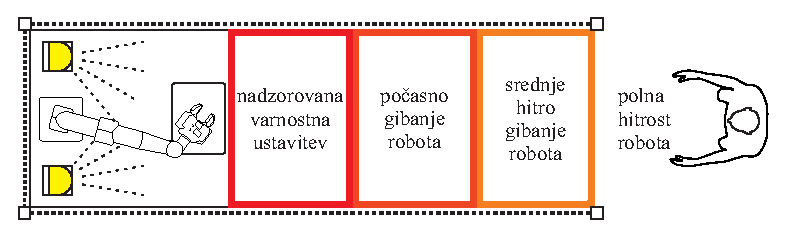
\includegraphics[width=\textwidth]{hc10_sdm.eps}
	\caption{Primer različnih področij hitrosti robota; bolj kot je področje oddaljeno, hitreje se robot lahko premika.}
	\label{fig:hc10_sdm}
\end{figure}

\subsection*{Izvedba naloge}

Pri tej nalogi boste definirali eno varnostno območje. če se bo v tem območju nahajala oseba, boste omejili gibanje robota na hitrost 50~mm/s, drugače pa se bo robot gibal s hitrostjo 250~mm/s. Za spremljanje prisotnosti človeka v varnostnem območju boste uporabili dodatni laserski skener proizvajalca SICK.

\subsubsection*{Nastavitev laserskega skenerja SICK TIM310}

V prvem delu naloge boste ustrezno sprogramili laserski skener. Pred programiranjem naprave se prepričajte, da je naprava fizično priklopljena na napajanje -- na senzorju sveti zelena LED. V programu, ki ste ga napisali v prejšnjem delu, popravite ukaz za hitrost linearnih premikov \textbf{SPEED} na \textbf{V=1500}.

Senzor priključite na računalnik preko USB kabla. Na računalniku se samodejno zažene programska oprema SOPAS, ki samodejno prepozna priključeno napravo. Za urejanje nastavitev je potrebno klikniti na ikono prepoznane naprave, ki je prikazana na sliki \ref{fig:hc10_sick1}.

\begin{figure}[!hbt]
	\centering
	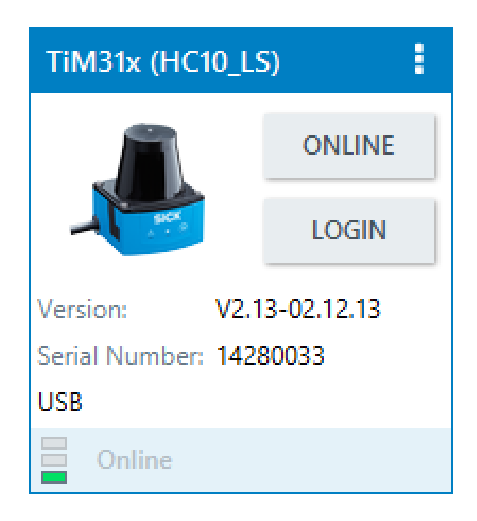
\includegraphics[width=0.3\textwidth]{hc10_sick1.eps}
	\caption{Prikaz prepoznane naprave znotraj programskega okolja SOPAS}
	\label{fig:hc10_sick1}
\end{figure}

Odpre se vam okno za urejanje nastavitev naprave, kjer se na levi strani nahaja drevesna struktura. Deli se na tri osnovne mape: \emph{Parameter}, \emph{Monitor} in \emph{Service}. Za prilagajanje delovanja senzorja je potrebno urediti nastavitve znotraj mape \textbf{Parameter} (slika \ref{fig:hc10_sick2}).

\begin{figure}[!hbt]
	\centering
	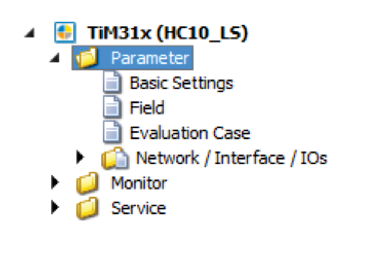
\includegraphics[width=0.3\textwidth]{hc10_sick2.eps}
	\caption{Drevesna struktura nastavitev laserskega skenerja}
	\label{fig:hc10_sick2}
\end{figure}

Najprej uredite ustrezno obliko območja znotraj katerega želimo, da senzor prepozna morebitno prisotnost. Območje naj bo po obliki in dimenziji približno enako polju, kot je prikazano na sliki \ref{fig:hc10_sick3}. Območje uredite z orodji, ki jih lahko opazimo na levi strani slike \ref{fig:hc10_sick3} (označena s številkami 1 -- 4).
\begin{itemize}
	\item Skupina orodij 1 je namenjena urejanju točk, na katerih temelji oblika polja. Prvo orodje je namenjeno dodajanju točk, drugo orodje omogoča urejanje že obstoječih točk, tretje orodje pa je namenjeno brisanju točk.
	\item Skupina orodij 2 je namenjena avtomatskemu izločanju objektov znotraj vidnega polja naprave.
	\item Skupina orodij 3 predstavlja izris prepoznanih objektov znotraj polja.
	\item Skupina orodij 4 predstavlja način prikaza polja naprave.
\end{itemize}

\begin{figure}[!hbt]
	\centering
	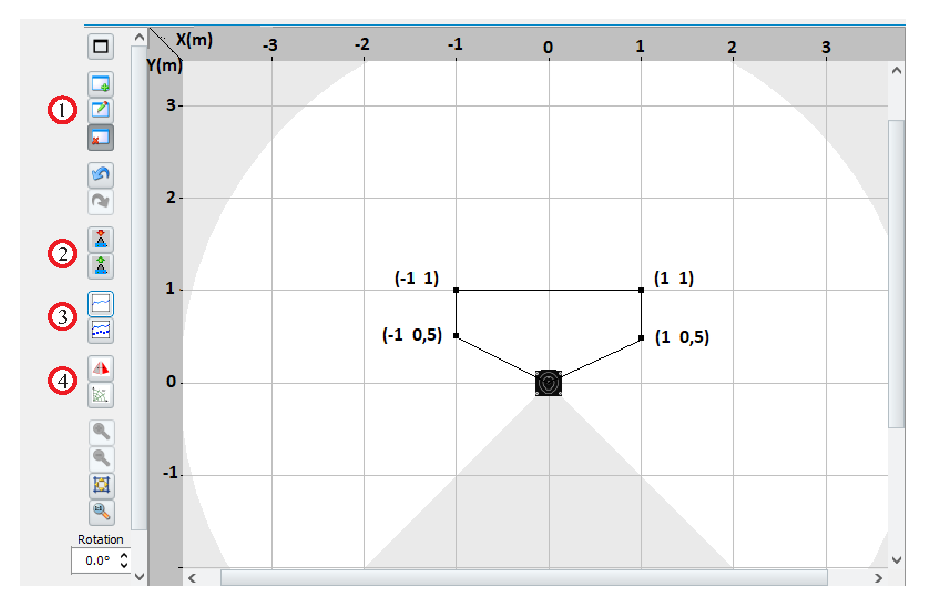
\includegraphics[width=0.9\textwidth]{hc10_sick3.eps}
	\caption{Okno za nastavljanje potrebne oblike varnostnega območja}
	\label{fig:hc10_sick3}
\end{figure}

Znotraj narisanega polja se definirajo tri varnostna območja, znotraj vsakega območja pa se spremlja morebitno prisotnost objektov. Vsako območje pro\v zi ustrezen digitalni izhod senzorja, ki je vezan naprej na FSU robotskega krmilnika. Pri vaji boste spremljali samo prisotnost osebe v srednjem območju.

Ko boste definirali ustrezno območje, definirajte tudi parametre znotraj zavihka \textbf{Evaluation Case}:
\begin{itemize}
	\item Duration time output - \v zelimo čim manjšo zakasnitev med tem, ko objekt ni več prisoten in ponovnim zagonom robota;
	\item Response time - \v zelimo, da se robot v čim krajšem času ustavi;
	\item Blanking size - \v zelimo, da senzor ne prepozna objektov manjših od 50 mm.
\end{itemize}

Z eksperimentalnim poiskušanjem poiščite ustrezne nastavitve senzorja.

Ko so vsi parametri ustrezno urejeni, zaprete okno za urejanje nastavitev naprave. Prikaže se nam opozorilo, če želimo spremembe shraniti na napravo. S tem, ko prenos potrdite, ste zaključili z nastavljanjem senzorja za prepoznavo prisotnosti. Iz senzorja izklopite USB kabel.

\subsection{Nastavitev robotskega krmilnika} \label{realni3}

V drugem delu boste ustrezno omejili hitrosti robota glede na informacijo iz laserskega skenerja. Omejitve hitrosti se nastavljajo v meniju \textbf{SAFETY FUNC.}, zavihek \textbf{SPEED LIMIT} (prikazano na sliki \ref{fig:hc10_speed1}). V tem zavihku lahko ustvarimo in nastavimo več datotek, ki omejujejo hitrost robota. Za to vajo boste ustvarili dve različni omejitvi hitrosti robota (dve datoteki): delovno hitrost ter hitrost pri interakciji (datoteka 1 in 2).

\begin{figure}[!hbt]
	\centering
	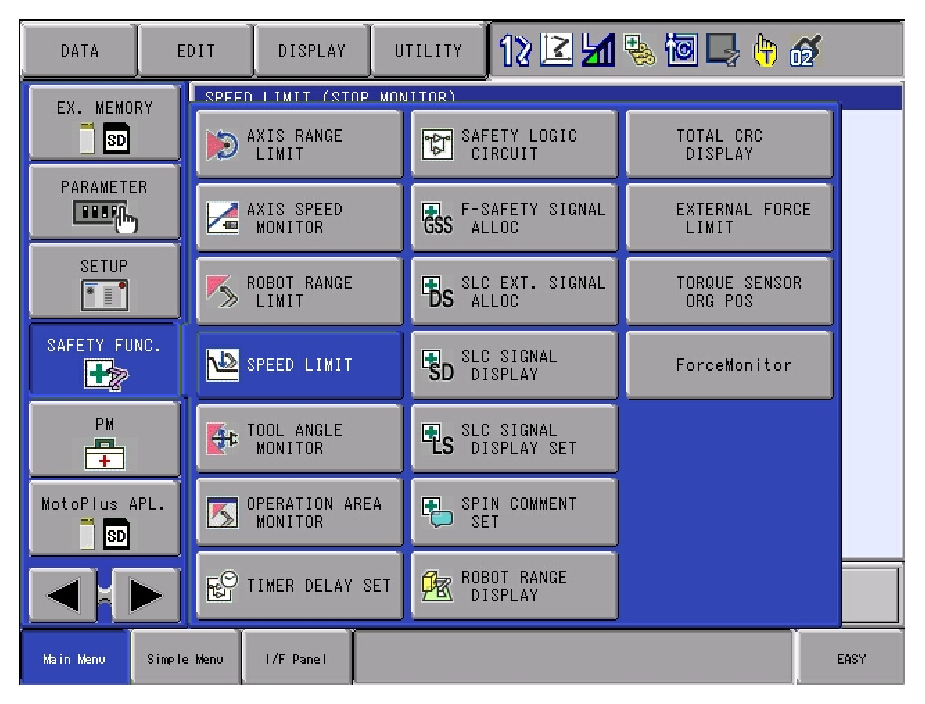
\includegraphics[width=0.7\textwidth]{hc10_speed1.eps}
	\caption{Meni Safety functions}
	\label{fig:hc10_speed1}
\end{figure}

Odpre se vam okno, ki je prikazano na sliki \ref{fig:hc10_speed2}. V tem zavihku lahko ustvarimo in nastavimo več datotek, ki omejujejo hitrost robota. Za to vajo boste ustvarili dve različni omejitvi hitrosti robota (dve datoteki): delovno hitrost ter hitrost pri interakciji (datoteka 1 in 2).

\begin{figure}[!hbt]
	\centering
	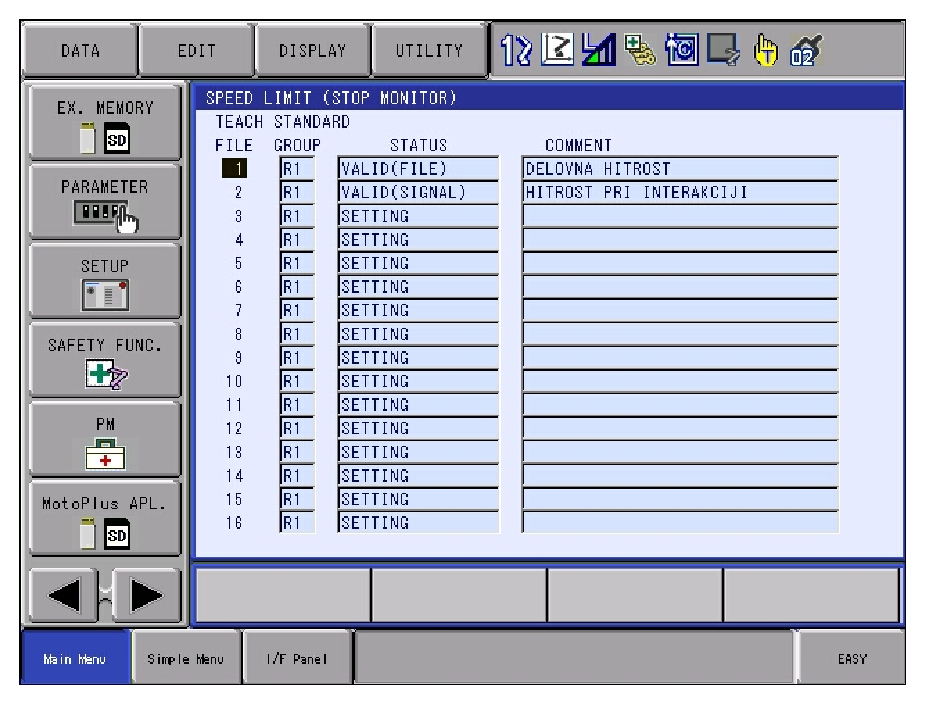
\includegraphics[width=0.7\textwidth]{hc10_speed2.eps}
	\caption{Zavihek Speed Limit}
	\label{fig:hc10_speed2}
\end{figure}

Delovno hitrost nastavite tako, da odprete prvo datoteko. S pomočjo puščic se postavimo v prvo vrstico in jo izberete s tipko \textbf{SELECT}. Odpre se vam okno, kot je prikazano na sliki \ref{fig:hc10_speed3}. V tem oknu morate ustrezno izpolniti polja \textbf{COMMENT}, \textbf{FILE VALID COND.}, \textbf{CTRL GROUP} ter \textbf{LIMIT SPEED}.

\begin{itemize}
	\item V polje \textbf{COMMENT} vpišete komentar datoteke (npr. delovna hitrost).
	\item V polju \textbf{FILE VALID COND.} nastavite, kdaj velja ta omejitev hitrosti. Lahko izbirate med \textbf{VALID}, ko omejitev velja vedno, \textbf{SIGNAL}, ko želite, da je omejitev hitrosti aktivna ob določenem pogoju (signalu), in {\textbf{INVALID}}, ko ne želite, da je omejitev aktivna. Pri tej hitrosti želite, da je omejitev vedno aktivna.
	\item V polju \textbf{CTRL GROUP} nastavite, za katerega robota velja omejitev hitrosti. V vašem primeru imate samo enega robota, zato nastavite na \textbf{R1}.
	\item V polju \textbf{LIMIT SPEED} definirate dejansko omejitev hitrosti. Za delovno hitrost nastavite omejitev na 250~mm/s.
\end{itemize}

Ostale nastavitve ostanejo nespremenjene. Nastavitve zapišete s pritiskom na gumb \textbf{READBACK} ter nato še \textbf{WRITE}. Pojavi se opozorilo, če želite posodobiti datotetko, na kar odgovorite z \textbf{YES}.

\begin{figure}[!hbt]
	\centering
	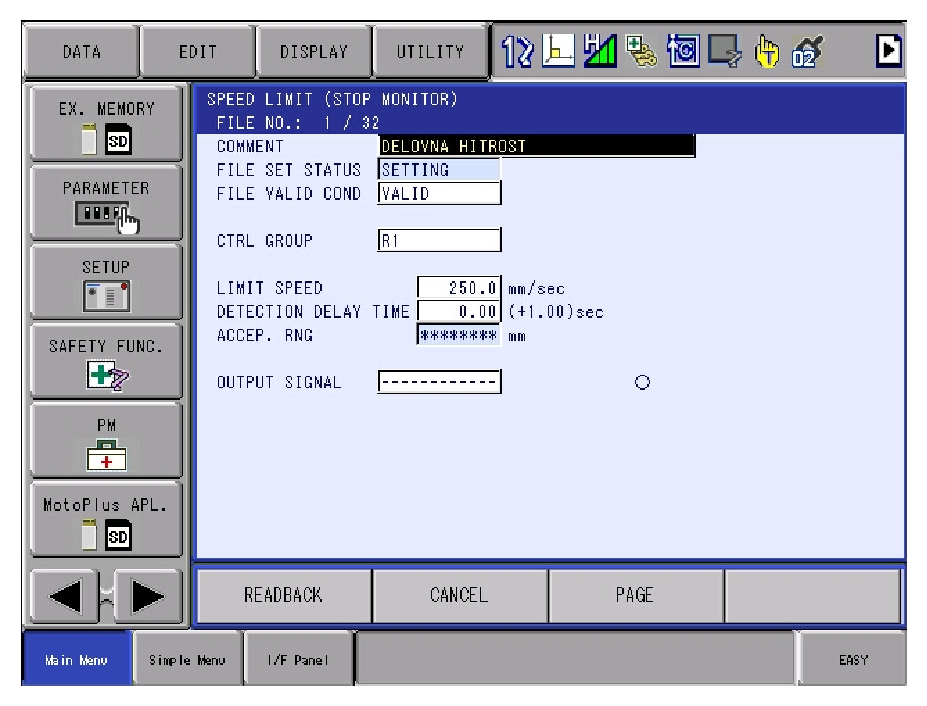
\includegraphics[width=0.7\textwidth]{hc10_speed3.eps}
	\caption{Nastavitve za delovno hitrost}
	\label{fig:hc10_speed3}
\end{figure}

Ko končate z nastavitvijo delovne hitrosti, nastavite še hitrost pri interakciji. V zavihku \textbf{SPEED LIMIT} se pomaknite na drugo vrstico in jo odprete s tipko \textbf{SELECT}. Odpre se vam okno prikazano na sliki \ref{fig:hc10_speed4}. Podobno kot pri nastavljanju delovne hitrosti moate tudi pri hitrosti interakcije ustrezno izpolniti polja \textbf{COMMENT}, \textbf{FILE VALID COND.}, \textbf{CTRL GROUP} ter \textbf{LIMIT SPEED}.

\begin{itemize}
	\item V polje \textbf{COMMENT} vpišete komentar datoteke (npr. hitrost pri interakciji).
	\item V polju \textbf{FILE VALID COND.} nastavite, kdaj velja ta omejitev hitrosti. Ta  omejitev naj bo aktivna takrat, ko laserski skener zazna osebo v svojem varnostnem območju, zato nastavite parameter na \textbf{SIGNAL}. Ob tem se vam pojavi dodatna možnost \textbf{INPUT SIGNAL}, kjer lahko definirate več pogojev oziroma signalov s poljubno logiko (\textbf{bit0} -- \textbf{bit4}). V vašem primeru gledate samo signal laserskega skenerja, ki je v robotskem krmilniku vezan na digitalni vhod  \textbf{FSBIN02( \#1)} z negativno logiko. Ta signal nastavite v polju \textbf{bit0}, kot je prikazano na sliki \ref{fig:hc10_speed4}. S parametrom \textbf{SET} nastavite negativno logiko (parameter nastavite na \emph{OFF}). Negativna logika pomeni to, da laserski skener postavi digitalni izhod na nizek nivo, ko zazna prisotnost osebe v varnostnem območju, v nasprotnem primeru pa je digitalni izhod postavljen na visok nivo. Parameter \textbf{STATUS} vam prikazuje trenutno vrednost digitalnega vhoda - poln krogec predstavlja logično 1, prazen krogec pa logično 0.
	\item V polju \textbf{CTRL GROUP} nastavite na \textbf{R1}.
	\item V polju \textbf{LIMIT SPEED} definirate dejansko omejitev hitrosti. Za hitrost ob potencialni interakciji nastavite omejitev na 50~mm/s.
\end{itemize}

Ostale nastavitve ostanejo nespremenjene. Nastavitve zapišete s pritiskom na gumb \textbf{READBACK} ter nato še \textbf{WRITE}. Pojavi se opozorilo, če želite posodbiti datotetko, na kar odgovorite z \textbf{YES}.

\begin{figure}[!hbt]
	\centering
	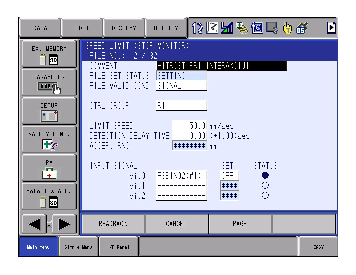
\includegraphics[width=0.7\textwidth]{hc10_speed4.eps}
	\caption{Nastavitve za hitrost pri interakciji}
	\label{fig:hc10_speed4}
\end{figure}

\subsection{Testiranje omejevanja hitrosti} \label{test3del}

Za testiranje funkcionalnosti omejevanja hitrosti izberite vaš program, ki ste ga napisali v II. delu. Poženite ga v \textbf{RUN} načinu: postavite se na začetek programa, ključ na učni enoti postavite na srednjo pozicijo, prižgite motorje s \textbf{SERVO ON READY} in pritisnete zeleni gumb na vrhu učne enote.

Za testiranje se odmaknite iz vidnega polja senzorja. Robot se mora premikati s hitrostjo 250~mm/s. Ko nekdo vstopi v varnostno območje senzorja, se mora hitrost robota opazno zmanjšati na 50~mm/s.

Na podoben način bi lahko definirali še omejitve hitrosti za ostali dve območji. Pri tem bi območje najbližje robotu (najbolj nevarno zaradi največje možnosti trka) zahtevalo vklop varnostno nadzorovane ustavitve.



